\documentclass[11pt]{article}

\usepackage[margin=0.85in]{geometry}
\usepackage[T1]{fontenc}
\usepackage{lmodern}
\usepackage{microtype}
\usepackage{amsmath,amssymb,mathtools}
\usepackage[dvipsnames]{xcolor}
\usepackage{hyperref}
\usepackage{parskip}
\usepackage{enumitem}
\usepackage{booktabs}
\usepackage{array}
\usepackage{tabularx}
\usepackage{titlesec}
\usepackage[most]{tcolorbox}
\usepackage{tikz}
\usetikzlibrary{arrows.meta,positioning,shapes.geometric,fit,calc,backgrounds}

\hypersetup{colorlinks=true,linkcolor=MidnightBlue,urlcolor=BrickRed,citecolor=OliveGreen}

\definecolor{rlblue}{HTML}{1D4ED8}
\definecolor{rlgreen}{HTML}{15803D}
\definecolor{rlorange}{HTML}{EA580C}
\definecolor{rlgold}{HTML}{CA8A04}
\definecolor{rlviolet}{HTML}{7C3AED}
\definecolor{rlgray}{HTML}{334155}
\definecolor{rlpaper}{HTML}{F8FAFC}

\titleformat{\section}{\Large\bfseries\color{rlblue}}{\thesection}{0.6em}{}
\titleformat{\subsection}{\large\bfseries\color{rlviolet}}{\thesubsection}{0.6em}{}

\setlist[itemize]{leftmargin=1.25em,itemsep=0.35em,topsep=0.35em}
\renewcommand{\arraystretch}{1.18}
\newcolumntype{Y}{>{\raggedright\arraybackslash}X}

\newcommand{\E}{\mathbb{E}}
\newcommand{\Var}{\mathrm{Var}}
\newcommand{\KL}{\mathrm{KL}}
\newcommand{\adv}{\hat{A}}
\DeclareMathOperator*{\argmax}{arg\,max}

\newtcolorbox{intuitionbox}[1][]{
  colback=blue!4!white,
  colframe=rlblue,
  boxrule=0.8pt,
  arc=2mm,
  title=Intuition,
  fonttitle=\bfseries,
  #1
}

\newtcolorbox{mathbox}[1][]{
  colback=orange!5!white,
  colframe=rlorange,
  boxrule=0.8pt,
  arc=2mm,
  title=Math Snapshot,
  fonttitle=\bfseries,
  #1
}

\newtcolorbox{takeawaybox}[1][]{
  colback=green!5!white,
  colframe=rlgreen,
  boxrule=0.8pt,
  arc=2mm,
  title=Takeaway,
  fonttitle=\bfseries,
  #1
}

\newtcolorbox{deepseekbox}[1][]{
  colback=violet!4!white,
  colframe=rlviolet,
  boxrule=0.8pt,
  arc=2mm,
  title=DeepSeekMath Lens,
  fonttitle=\bfseries,
  #1
}

\title{Reinforcement Learning for Understanding DeepSeekMath\\
\large From Bandits and Bellman Equations to PPO, DPO, and GRPO}
\author{Intuitive study note}
\date{April 2026}

\begin{document}

\maketitle

\begin{intuitionbox}
Reinforcement learning is the study of how an agent can learn by \emph{trying actions}, \emph{seeing outcomes}, and then \emph{shifting probability mass toward decisions that pay off more often}. For LLM reasoning, the actions are tokens, the ``environment'' is the prompt plus generated prefix, and the reward often arrives only at the end.
\end{intuitionbox}

\begin{center}
\small All figures in this note are original schematic redrawings rather than copied images. They are inspired by canonical expositions such as Sutton and Barto's textbook, the DQN paper, PPO/TRPO material, OpenAI Spinning Up, and the DeepSeekMath paper.
\end{center}

\tableofcontents

\section{Why RL Feels Different}

If supervised learning is ``copy the labeled answer,'' reinforcement learning is ``sample a behavior, score the outcome, and then make better-scoring behaviors more likely next time.'' That single shift explains most of the field.

RL feels hard for three reasons:

\begin{itemize}
  \item The agent usually sees \emph{delayed rewards}, so it must assign credit backward through a trajectory.
  \item The agent must \emph{explore}, so it cannot only repeat what already looks best.
  \item The data distribution depends on the current policy, so learning changes the future data.
\end{itemize}

\begin{takeawaybox}
No short note can literally enumerate every RL variant that exists today. The useful compression is to understand the main \emph{families}: bandits, dynamic programming, Monte Carlo, temporal-difference methods, value-based deep RL, policy gradients, actor-critic methods, model-based RL, offline RL, and modern LLM post-training methods such as DPO, PPO, and GRPO.
\end{takeawaybox}

\section{Start Even Smaller: Bandits}

The multi-armed bandit is RL with the memory removed. You repeatedly choose one of several actions, immediately observe a reward, and want to maximize long-run payoff.

\begin{intuitionbox}
Imagine choosing between three study habits each evening: flash cards, worked examples, or rereading notes. There is no changing state, only a repeated choice and a reward the next day. That is a bandit, not a full RL problem.
\end{intuitionbox}

The central tension is \textbf{exploration vs. exploitation}:

\begin{itemize}
  \item \textbf{Exploitation}: choose the arm that currently looks best.
  \item \textbf{Exploration}: try uncertain arms because your estimate might be wrong.
\end{itemize}

Classic bandit rules already preview later RL ideas:

\begin{itemize}
  \item \textbf{$\varepsilon$-greedy}: usually take the current best action, but sometimes explore randomly.
  \item \textbf{UCB}: prefer actions with high estimated reward \emph{and} high uncertainty.
  \item \textbf{Thompson sampling}: sample from your posterior belief and act according to that sampled world.
\end{itemize}

\begin{mathbox}
The simplest action-value update is
\[
Q_{n+1}(a) = Q_n(a) + \alpha\bigl(R_n - Q_n(a)\bigr).
\]
This says: \emph{move your old estimate toward the new reward}. Nearly all RL updates keep this same skeleton: old estimate plus learning rate times prediction error.
\end{mathbox}

Bandits teach the first durable lesson of RL: \emph{good control requires both reward estimates and uncertainty management}.

\section{From Bandits to Full RL: Markov Decision Processes}

Bandits have no state. Full RL adds dynamics: your action changes what situation you face next. The standard model is the \textbf{Markov Decision Process (MDP)}:

\[
(\mathcal S, \mathcal A, P, R, \gamma).
\]

Here $\mathcal S$ is the state space, $\mathcal A$ the action space, $P$ the transition rule, $R$ the reward rule, and $\gamma \in [0,1)$ the discount factor.

\subsection{The Smallest RL Picture}

\begin{figure}[t]
\centering
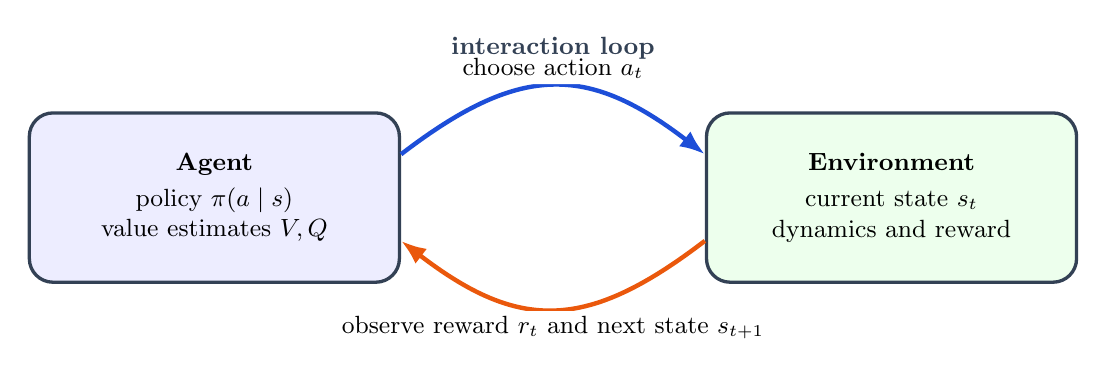
\begin{tikzpicture}[
  x=1cm,
  y=1cm,
  font=\small,
  card/.style={rectangle, rounded corners=3mm, draw=rlgray, very thick, fill=white, minimum width=4.7cm, minimum height=2.15cm, align=center},
  loop/.style={-{Latex[length=3.2mm]}, ultra thick},
  lab/.style={fill=white, inner sep=2pt, rounded corners=1.5mm}
]
  \node[card, fill=blue!7!white] (agent) at (0,0) {\textbf{Agent}\\[2pt]policy $\pi(a\mid s)$\\value estimates $V,Q$};
  \node[card, fill=green!7!white] (env) at (8.6,0) {\textbf{Environment}\\[2pt]current state $s_t$\\dynamics and reward};

  \draw[loop, draw=rlblue] ($(agent.east)+(0,0.55)$) .. controls +(1.5,1.15) and +(-1.5,1.15) .. node[lab, above] {choose action $a_t$} ($(env.west)+(0,0.55)$);
  \draw[loop, draw=rlorange] ($(env.west)+(0,-0.55)$) .. controls +(-1.5,-1.15) and +(1.5,-1.15) .. node[lab, below] {observe reward $r_t$ and next state $s_{t+1}$} ($(agent.east)+(0,-0.55)$);
  \node[font=\bfseries\small, color=rlgray] at (4.3,1.9) {interaction loop};
\end{tikzpicture}
\caption{The basic agent--environment loop. This is the common core behind chess engines, robot control, Atari agents, and LLM post-training.}
\end{figure}

  If the current state contains all information needed for prediction, we call the problem \emph{Markov}. Then a policy $\pi(a\mid s)$ fully specifies behavior.

  The return from time $t$ is
  \[
  G_t = r_t + \gamma r_{t+1} + \gamma^2 r_{t+2} + \cdots.
  \]

  Why discount? Three intuitive reasons:

  \begin{itemize}
    \item It makes ``reward now'' worth more than ``reward much later.''
    \item It helps infinite-horizon sums stay finite.
    \item It stabilizes planning by reducing how far tiny errors propagate.
  \end{itemize}

  Two functions dominate RL theory:

  \begin{itemize}
    \item \textbf{State value} $V^\pi(s)$: expected return if you start in state $s$ and then follow policy $\pi$.
    \item \textbf{Action value} $Q^\pi(s,a)$: expected return if you take action $a$ in state $s$ and then follow $\pi$.
  \end{itemize}

  \begin{mathbox}
  The Bellman expectation equations are the self-consistency laws of RL:
  \[
  V^\pi(s)=\sum_a \pi(a\mid s) \sum_{s',r} P(s',r\mid s,a)\,[r+\gamma V^\pi(s')],
  \]
  \[
  Q^\pi(s,a)=\sum_{s',r} P(s',r\mid s,a)\Bigl[r+\gamma \sum_{a'}\pi(a'\mid s')Q^\pi(s',a')\Bigr].
  \]
  The deep idea is that a value function equals \emph{immediate reward plus discounted value of what comes next}.
  \end{mathbox}

  \subsection{One Running Example}

  Picture a maze. The agent receives $-0.01$ each step, $+1$ at the exit, and maybe $-1$ for stepping into lava. Now every algorithm in RL is trying to answer some version of one question:

  \begin{center}
  \emph{How should I update my beliefs so that future action choices lead me to the exit faster and more reliably?}
  \end{center}

  \section{How Classical RL Learns}

  The historical flow is simple:

  \begin{itemize}
    \item If you know the model exactly, you can plan with \textbf{dynamic programming}.
    \item If you can run episodes but do not know the model, you can average outcomes with \textbf{Monte Carlo}.
    \item If you want to learn online and bootstrap from current estimates, you use \textbf{temporal-difference learning}.
  \end{itemize}

  \subsection{Dynamic Programming}

  Dynamic programming assumes the transition model $P$ is known. Then you can repeatedly evaluate and improve a policy.

  The two classical loops are:

  \begin{itemize}
    \item \textbf{Policy iteration}: evaluate $\pi$, then greedify it.
    \item \textbf{Value iteration}: repeatedly apply the Bellman optimality backup until values stabilize.
  \end{itemize}

  \begin{intuitionbox}
  Dynamic programming is like having the full rules of a board game and computing consequences before acting. It is powerful, but in many real problems you do not know the transition table or the state space is too large.
  \end{intuitionbox}

  \subsection{Monte Carlo}

  Monte Carlo (MC) waits until an episode ends, then uses the observed return to update values. It does not bootstrap from current value estimates.

  Pros: unbiased with enough samples and conceptually simple.\newline
  Cons: high variance and awkward for long episodes because you must wait until the end.

  \subsection{Temporal-Difference Learning}

  TD learning updates early, before the episode ends. The basic TD(0) update is
  \[
  V(s_t) \leftarrow V(s_t) + \alpha\Bigl(r_t + \gamma V(s_{t+1}) - V(s_t)\Bigr).
  \]

  The quantity in parentheses is the \textbf{TD error}. It is the same basic form as the bandit prediction error, except now the target includes a bootstrap term from the next state's current value estimate.

  \begin{figure}[t]
  \centering
  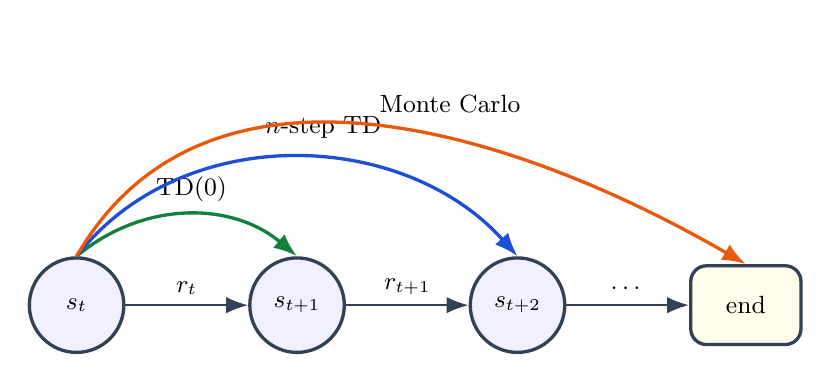
\begin{tikzpicture}[
    x=1cm,
    y=1cm,
    font=\small,
    state/.style={circle, draw=rlgray, very thick, minimum size=12mm, fill=white},
    term/.style={rectangle, rounded corners=2mm, draw=rlgray, very thick, minimum width=14mm, minimum height=10mm, fill=yellow!8!white},
    edge/.style={-{Latex[length=2.8mm]}, thick, draw=rlgray},
    callout/.style={fill=white, inner sep=2pt, rounded corners=1.2mm}
  ]
    \node[state, fill=blue!6!white] (s0) at (0,0) {$s_t$};
    \node[state, fill=blue!6!white] (s1) at (2.8,0) {$s_{t+1}$};
    \node[state, fill=blue!6!white] (s2) at (5.6,0) {$s_{t+2}$};
    \node[term] (st) at (8.5,0) {end};

    \draw[edge] (s0) -- node[above] {$r_t$} (s1);
    \draw[edge] (s1) -- node[above] {$r_{t+1}$} (s2);
    \draw[edge] (s2) -- node[above] {$\cdots$} (st);

    \draw[-{Latex[length=3mm]}, very thick, draw=rlgreen] (s0.north) to[out=40,in=140] node[callout, pos=0.52, above=2pt] {TD(0)} (s1.north);
    \draw[-{Latex[length=3mm]}, very thick, draw=rlblue] (s0.north) to[out=52,in=132] node[callout, pos=0.56, above=5pt] {$n$-step TD} (s2.north);
    \draw[-{Latex[length=3mm]}, very thick, draw=rlorange] (s0.north) to[out=60,in=150] node[callout, pos=0.6, above=7pt] {Monte Carlo} (st.north);
  \end{tikzpicture}
  \caption{How backup depth changes the algorithm. TD updates after one step, Monte Carlo waits until termination, and $n$-step methods interpolate between them.}
  \end{figure}

  \begin{takeawaybox}
  Monte Carlo learns from complete outcomes. TD learns from partial outcomes plus current guesses. That single difference creates the bias--variance trade-off at the heart of classical RL.
  \end{takeawaybox}

  \subsection{SARSA and Q-Learning}

  Once we move from prediction to control, the central object becomes $Q(s,a)$.

  \textbf{SARSA} is on-policy:
  \[
  Q(s_t,a_t) \leftarrow Q(s_t,a_t) + \alpha\bigl[r_t + \gamma Q(s_{t+1},a_{t+1}) - Q(s_t,a_t)\bigr].
  \]

  \textbf{Q-learning} is off-policy:
  \[
  Q(s_t,a_t) \leftarrow Q(s_t,a_t) + \alpha\bigl[r_t + \gamma \max_{a'} Q(s_{t+1},a') - Q(s_t,a_t)\bigr].
  \]

  The intuitive difference is clean:

  \begin{itemize}
    \item \textbf{SARSA} learns about the action you actually took next. It is usually more conservative.
    \item \textbf{Q-learning} learns about the best next action according to your current estimate. It is more optimistic and often more aggressive.
  \end{itemize}

  \begin{table}[t]
  \centering
  \small
  \begin{tabularx}{\linewidth}{@{}lYYY@{}}
  \toprule
  Method & What it assumes & Main strength & Main weakness \\
  \midrule
  Dynamic programming & Known transition model & Exact planning on small MDPs & Unrealistic for most large unknown environments \\
  Monte Carlo & Episodic rollouts & Simple and unbiased in the limit & High variance, must wait for episode end \\
  TD(0), TD($\lambda$) & Streaming experience & Data efficient, online updates & Bootstrapping can propagate bad estimates \\
  SARSA & On-policy control & Safer under exploratory behavior & Can be conservative \\
  Q-learning & Off-policy control & Strong asymptotic target, greedy improvement & Can be unstable with function approximation \\
  \bottomrule
  \end{tabularx}
  \caption{The classical RL toolbox. These methods are still conceptually central even when modern implementations use neural networks.}
  \end{table}

  \section{When Neural Networks Enter: Deep RL}

  Tabular methods break when the state space is huge. You cannot store one value per pixel image, robot pose history, or token prefix. The fix is function approximation: use a neural network to approximate values or policies.

  \begin{figure}[t]
  \centering
  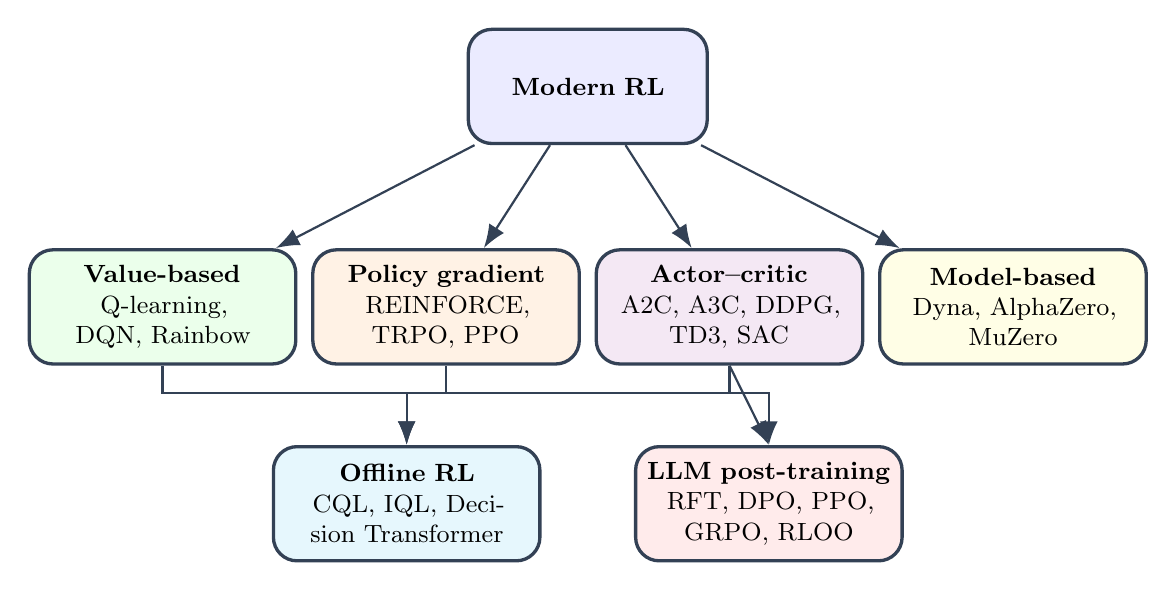
\begin{tikzpicture}[
    x=1cm,
    y=1cm,
    font=\small,
    family/.style={rectangle, rounded corners=3mm, draw=rlgray, very thick, minimum height=1.45cm, text width=3.15cm, align=center, fill=white},
    link/.style={-{Latex[length=3mm]}, thick, draw=rlgray}
  ]
    \node[family, fill=blue!8!white, text width=2.8cm] (root) at (0,0) {\textbf{Modern RL}};
    \node[family, fill=green!8!white] (value) at (-5.4,-2.8) {\textbf{Value-based}\\Q-learning, DQN, Rainbow};
    \node[family, fill=orange!10!white] (policy) at (-1.8,-2.8) {\textbf{Policy gradient}\\REINFORCE, TRPO, PPO};
    \node[family, fill=violet!9!white] (ac) at (1.8,-2.8) {\textbf{Actor--critic}\\A2C, A3C, DDPG, TD3, SAC};
    \node[family, fill=yellow!10!white] (model) at (5.4,-2.8) {\textbf{Model-based}\\Dyna, AlphaZero,\\MuZero};
    \node[family, fill=cyan!10!white] (offline) at (-2.3,-5.3) {\textbf{Offline RL}\\CQL, IQL, Decision Transformer};
    \node[family, fill=red!8!white] (llm) at (2.3,-5.3) {\textbf{LLM post-training}\\RFT, DPO, PPO, GRPO, RLOO};

    \draw[link] (root) -- (value);
    \draw[link] (root) -- (policy);
    \draw[link] (root) -- (ac);
    \draw[link] (root) -- (model);
    \draw[link] (policy.south) -- ++(0,-0.35) -| (llm.north);
    \draw[link] (ac.south) -- (llm.north);
    \draw[link] (value.south) -- ++(0,-0.35) -| (offline.north);
    \draw[link] (ac.south) -- ++(0,-0.35) -| (offline.north);
  \end{tikzpicture}
  \caption{A family tree of the major modern RL directions. This is a conceptual map, not an exhaustive list of every named variant.}
  \end{figure}

  \subsection{DQN and the Value-Based Deep RL Line}

  Deep Q-Networks (DQN) combine Q-learning with a neural network. The network receives a state and outputs values for actions. Two stabilizing ideas made DQN practical on Atari \cite{mnih2015}:

  \begin{itemize}
    \item \textbf{Replay buffer}: store past transitions and train on shuffled minibatches so updates are less correlated.
    \item \textbf{Target network}: use a slowly updated copy of the Q-network to build training targets.
  \end{itemize}

  \begin{figure}[t]
  \centering
  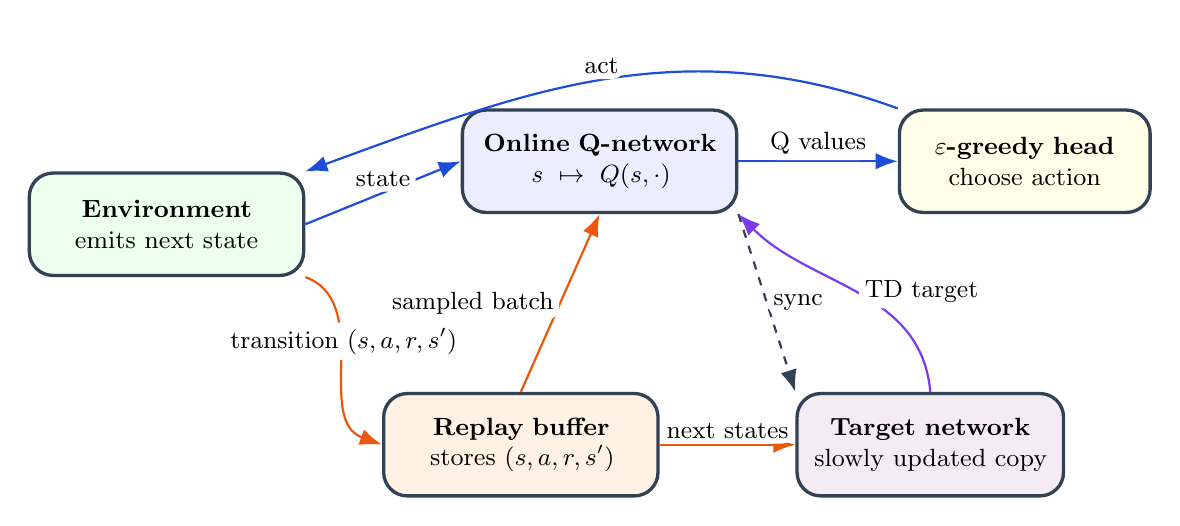
\begin{tikzpicture}[
    x=1cm,
    y=1cm,
    font=\small,
    box/.style={rectangle, rounded corners=3mm, draw=rlgray, very thick, minimum height=1.3cm, text width=3.25cm, align=center, fill=white},
    link/.style={-{Latex[length=2.8mm]}, thick, draw=rlblue},
    back/.style={-{Latex[length=2.8mm]}, thick, draw=rlorange},
    sync/.style={-{Latex[length=2.8mm]}, thick, dashed, draw=rlgray},
    lab/.style={fill=white, inner sep=2pt, rounded corners=1.5mm}
  ]
    \node[box, fill=green!7!white] (env) at (-1.5,0.8) {\textbf{Environment}\\emits next state};
    \node[box, fill=blue!7!white] (qnet) at (4.0,1.6) {\textbf{Online Q-network}\\$s \mapsto Q(s,\cdot)$};
    \node[box, fill=yellow!9!white, text width=2.95cm] (action) at (9.4,1.6) {\textbf{$\varepsilon$-greedy head}\\choose action};
    \node[box, fill=orange!10!white] (replay) at (3.0,-2.0) {\textbf{Replay buffer}\\stores $(s,a,r,s')$};
    \node[box, fill=violet!8!white, text width=3.15cm] (target) at (8.2,-2.0) {\textbf{Target network}\\slowly updated copy};

    \draw[link] (env.east) -- node[lab, above] {state} (qnet.west);
    \draw[link] (qnet.east) -- node[lab, above] {Q values} (action.west);
    \draw[link] (action.north west) to[out=160,in=20] node[lab, above] {act} (env.north east);
    \draw[back] (env.south east) to[out=-20,in=160] node[lab, above] {transition $(s,a,r,s')$} (replay.west);
    \draw[back] (replay.north) -- node[lab, left] {sampled batch} (qnet.south);
    \draw[back] (replay.east) -- node[lab, above] {next states} (target.west);
    \draw[sync] (qnet.south east) -- node[lab, right] {sync} (target.north west);
    \draw[link, draw=rlviolet] (target.north) to[out=95,in=-45] node[lab, right] {TD target} (qnet.south east);
  \end{tikzpicture}
  \caption{Original schematic of the DQN training loop, inspired by the stabilizing ideas in the Atari DQN line.}
  \end{figure}

  Important descendants include:

  \begin{itemize}
    \item \textbf{Double DQN}: reduce overestimation bias.
    \item \textbf{Dueling DQN}: separately represent state value and action advantage.
    \item \textbf{Prioritized replay}: sample more informative transitions more often.
    \item \textbf{Rainbow}: combine the strongest ingredients into one agent.
  \end{itemize}

  \subsection{Policy Gradient: Optimize the Policy Directly}

  Value-based methods choose actions by maximizing a learned value. Policy-gradient methods learn a parameterized policy directly.

  The canonical score-function result behind REINFORCE is
  \[
  \nabla_\theta J(\theta) = \E\Biggl[\sum_t G_t\, \nabla_\theta \log \pi_\theta(a_t\mid s_t)\Biggr].
  \]

  The intuition is wonderfully simple:

  \begin{itemize}
    \item If a trajectory turned out well, increase the log-probability of the actions that produced it.
    \item If a trajectory turned out badly, decrease those probabilities.
  \end{itemize}

  \begin{intuitionbox}
  REINFORCE says: \emph{do more of what lucky trajectories did}. The problem is variance. A single lucky episode can shout too loudly. This is why later methods add baselines, critics, clipping, and trust regions.
  \end{intuitionbox}

  \subsection{Actor--Critic}

  Actor--critic methods split the job:

  \begin{itemize}
    \item The \textbf{actor} is the policy $\pi_\theta$.
    \item The \textbf{critic} estimates values and provides a lower-variance training signal.
  \end{itemize}

  The key quantity is the \textbf{advantage}
  \[
  A^\pi(s,a) = Q^\pi(s,a) - V^\pi(s),
  \]

  which answers: \emph{how much better was this action than my baseline expectation in this state?}

  This idea powers A2C, A3C, GAE, DDPG, TD3, and SAC.

  \begin{itemize}
    \item \textbf{A2C/A3C}: synchronous or asynchronous actor--critic for faster parallel learning.
    \item \textbf{GAE}: smooth bias--variance trade-off for advantage estimation \cite{gae}.
    \item \textbf{DDPG / TD3}: deterministic actor--critic methods for continuous control.
    \item \textbf{SAC}: maximize reward \emph{and} entropy, so the policy stays stochastic and exploratory.
  \end{itemize}

  \subsection{Why PPO Became So Popular}

  TRPO said: update the policy, but do not move too far in one step. PPO kept that spirit with a simpler clipped objective \cite{ppo}:

  \[
  L^{\mathrm{PPO}}(\theta)=\E\bigl[\min(r_t(\theta)\adv_t,\, \mathrm{clip}(r_t(\theta),1-\varepsilon,1+\varepsilon)\adv_t)\bigr],
  \]

  where $r_t(\theta)=\pi_\theta(a_t\mid s_t)/\pi_{\mathrm{old}}(a_t\mid s_t)$.

  \begin{figure}[t]
  \centering
  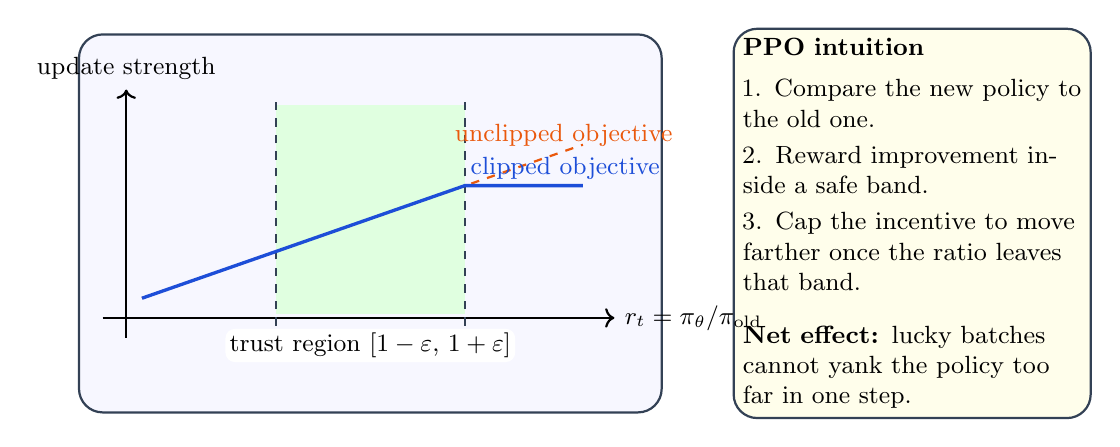
\begin{tikzpicture}[
    x=1cm,
    y=1cm,
    font=\small,
    panel/.style={rectangle, rounded corners=3mm, draw=rlgray, thick, fill=white}
  ]
    \node[panel, fill=blue!3!white, minimum width=7.4cm, minimum height=4.8cm] (plotbg) at (0,0) {};
    \node[panel, fill=yellow!8!white, text width=4.3cm, minimum height=4.8cm, align=left, anchor=west] (callout) at (4.6,0) {\textbf{PPO intuition}\\[4pt]
    1. Compare the new policy to the old one.\\[2pt]
    2. Reward improvement inside a safe band.\\[2pt]
    3. Cap the incentive to move farther once the ratio leaves that band.\\[8pt]
    \textbf{Net effect:} lucky batches cannot yank the policy too far in one step.};

    \draw[->, thick] (-3.1,-1.45) -- (-3.1,1.7) node[above] {update strength};
    \draw[->, thick] (-3.4,-1.2) -- (3.1,-1.2) node[right] {$r_t = \pi_\theta/\pi_{\mathrm{old}}$};
    \fill[green!12] (-1.2,-1.15) rectangle (1.2,1.5);
    \draw[dashed, thick, color=rlgray] (-1.2,-1.3) -- (-1.2,1.55);
    \draw[dashed, thick, color=rlgray] (1.2,-1.3) -- (1.2,1.55);
    \node[fill=white, inner sep=1.5pt, rounded corners=1.2mm] at (0,-1.55) {trust region $[1-\varepsilon,\,1+\varepsilon]$};

    \draw[thick, color=rlorange, dashed] (-2.9,-0.95) -- (2.7,1.0);
    \draw[very thick, color=rlblue] (-2.9,-0.95) -- (1.2,0.48) -- (2.7,0.48);
    \node[color=rlorange, anchor=west] at (0.95,1.12) {unclipped objective};
    \node[color=rlblue, anchor=west] at (1.15,0.7) {clipped objective};
  \end{tikzpicture}
  \caption{PPO's core intuition: do not let one update overreact to a lucky batch. The clipping acts like a seat belt for policy gradients.}
  \end{figure}

  PPO became popular because it is:

  \begin{itemize}
    \item simpler than TRPO,
    \item more stable than raw policy gradient,
    \item flexible enough for robotics, games, and later RLHF-style LLM training.
  \end{itemize}

  \subsection{Other Major Modern Directions}

  Beyond DQN and PPO, the main modern branches are:

  \begin{itemize}
    \item \textbf{Model-based RL}: learn or use a world model, then plan inside it. Dyna pioneered the idea; AlphaZero and MuZero made it famous in high-performance planning systems.
    \item \textbf{Offline RL}: learn from a fixed logged dataset without new interaction. Representative ideas include conservative value learning (CQL), implicit Q-learning (IQL), and sequence-model views such as Decision Transformer.
    \item \textbf{Hierarchical and multi-agent RL}: decompose long-horizon behavior into skills or coordinate multiple agents.
  \end{itemize}

  \section{A Mental Map of the Major RL Families}

  \begin{table}[t]
  \centering
  \small
  \begin{tabularx}{\linewidth}{@{}lYY@{}}
  \toprule
  Family & Representative algorithms & Best intuition \\
  \midrule
  Bandits & $\varepsilon$-greedy, UCB, Thompson sampling & Learn rewards under uncertainty when there is no state transition \\
  Planning with known model & Policy iteration, value iteration & Compute consequences before acting \\
  Model-free prediction / control & MC, TD, SARSA, Q-learning & Learn values from trial and error \\
  Value-based deep RL & DQN, Double DQN, Rainbow & Use a neural critic to tell actions how good they are \\
  Policy-based RL & REINFORCE, TRPO, PPO & Push probability mass directly toward better trajectories \\
  Actor--critic & A2C, A3C, DDPG, TD3, SAC & Actor chooses, critic judges \\
  Model-based RL & Dyna, AlphaZero, MuZero & Spend computation on imagination and planning \\
  Offline RL & CQL, IQL, Decision Transformer & Learn from logs while avoiding unsupported actions \\
  LLM RL / alignment & RFT, DPO, PPO, GRPO, RLOO & Reweight sampled completions using preference or reward signals \\
  \bottomrule
  \end{tabularx}
  \caption{The shortest honest overview of ``all the RL algorithms we have now'' is really a map of families and their representative members.}
  \end{table}

  \section{LLMs as Reinforcement Learning Agents}

  An LLM can be viewed as an episodic RL policy:

  \begin{itemize}
    \item \textbf{State}: the prompt plus the tokens generated so far.
    \item \textbf{Action}: the next token.
    \item \textbf{Episode}: one completion.
    \item \textbf{Reward}: a score for helpfulness, correctness, preference, safety, or final answer quality.
  \end{itemize}

  This is both familiar and strange:

  \begin{itemize}
    \item familiar, because it is still a policy over actions;
    \item strange, because the action space is huge, rewards are sparse, and one bad update can destroy useful language behavior.
  \end{itemize}

  That is why LLM RL almost always includes \textbf{regularization toward a reference policy}, often the supervised fine-tuned model. In practice, the model is allowed to improve, but not to wander arbitrarily far.

  \subsection{The Main LLM Post-Training Methods}

  DeepSeekMath gives a useful unifying lens: every post-training method can be understood by three ingredients.

  \begin{enumerate}
    \item Where does the data come from?
    \item What acts as the reward signal?
    \item How do we convert that signal into a gradient coefficient? 
  \end{enumerate}

  \begin{table}[t]
  \centering
  \small
  \begin{tabularx}{\linewidth}{@{}lYYYY@{}}
  \toprule
  Method & Data source & Reward signal & What it updates & Intuition \\
  \midrule
  SFT & Human demonstrations & implicit human choice & policy & imitate good behavior \\
  RFT & Sampled completions, keep the correct ones & rule-based correctness or filtering & policy & train only on accepted outputs \\
  Online RFT & Completions from the current policy & rule-based correctness & policy & keep refreshing the accepted set online \\
  DPO & Preference pairs & pairwise winner vs. loser & policy & make preferred completions more likely without an explicit reward model \\
  PPO & Online samples from current policy & reward model $+$ critic-based advantage & policy and critic & RLHF with trust-region style updates \\
  GRPO & Online groups of samples for the same prompt & reward model with group-relative normalization & policy only & compare completions against each other instead of training a separate critic \\
  \bottomrule
  \end{tabularx}
  \caption{A useful LLM-alignment map, following the unified perspective emphasized in DeepSeekMath.}
  \end{table}

  What about newer names such as IPO, ORPO, SimPO, KTO, RLOO, ReMax, or RAFT? They mostly modify one of the same axes: the data source, the reward/preference signal, or the exact form of the gradient coefficient. The family structure matters more than memorizing every acronym.

  \section{Why DeepSeekMath Uses GRPO}

  DeepSeekMath is about mathematical reasoning, so the RL question becomes:

  \begin{center}
  \emph{Given several candidate solutions to the same math problem, how do we reinforce the reasoning patterns that look better without paying the full memory cost of PPO?}
  \end{center}

  Their answer is \textbf{Group Relative Policy Optimization (GRPO)} \cite{deepseekmath}.

  \subsection{From PPO to GRPO}

  In LLM PPO, you typically need:

  \begin{itemize}
    \item a \textbf{policy model} to generate text,
    \item a \textbf{reward model} to score text,
    \item a \textbf{value model / critic} to estimate advantages,
    \item a \textbf{reference model} to supply a KL penalty.
  \end{itemize}

  That critic is expensive. Worse, LLM rewards are often sparse: a long completion may only receive a useful reward at the end, so token-level value estimation is awkward.

  GRPO removes the critic. Instead, for one question $q$, sample a group of outputs
  \[
  \{o_1,o_2,\dots,o_G\},
  \]

  score them with a reward model, and normalize \emph{within the group}:
  \[
  \tilde r_i = \frac{r_i - \mathrm{mean}(\mathbf r)}{\mathrm{std}(\mathbf r)}.
  \]

  For outcome supervision, every token in output $o_i$ receives the same advantage signal $\adv_{i,t}=\tilde r_i$.

  \begin{deepseekbox}
  The key intuition is comparative: a reward model is usually better at saying \emph{which of these completions is better for the same question} than at assigning an absolutely calibrated global score. GRPO leans into that fact.
  \end{deepseekbox}

  \begin{figure}[t]
  \centering
  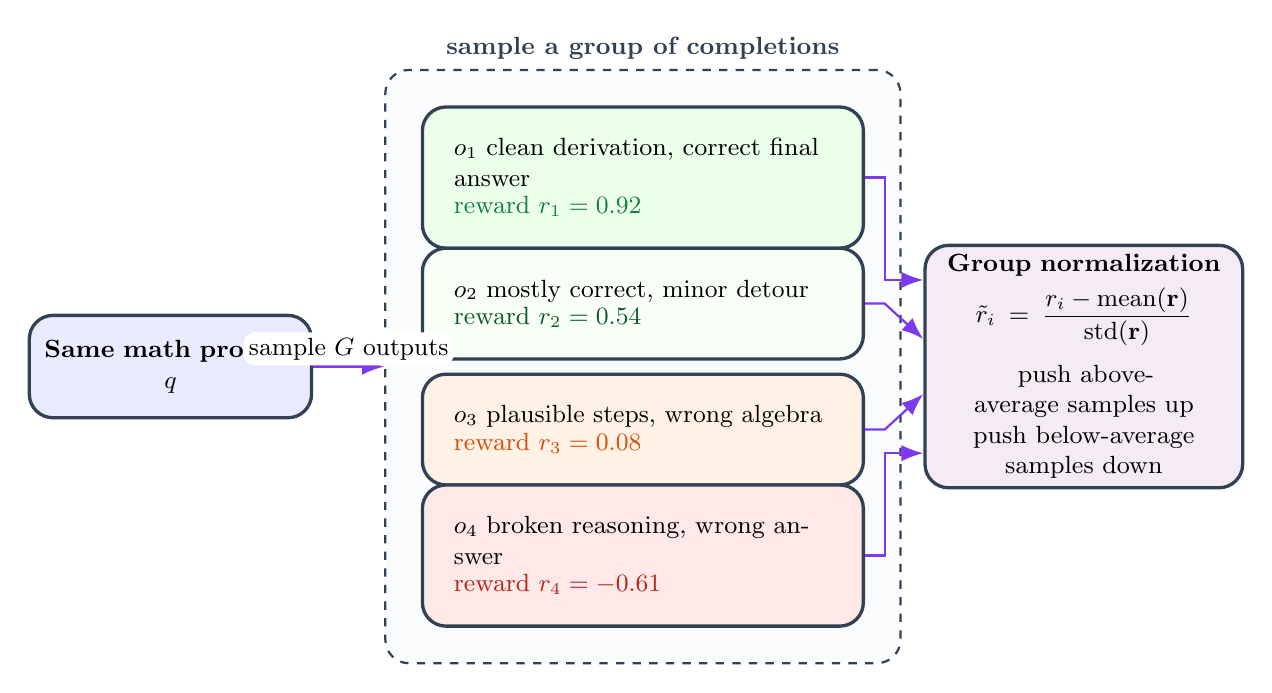
\begin{tikzpicture}[
    x=1cm,
    y=1cm,
    font=\small,
    box/.style={rectangle, rounded corners=3mm, draw=rlgray, very thick, minimum height=1.3cm, text width=3.35cm, align=center, fill=white},
    sol/.style={rectangle, rounded corners=3mm, draw=rlgray, very thick, text width=4.8cm, minimum height=1.05cm, align=left, fill=white, inner sep=4mm},
    link/.style={-{Latex[length=2.8mm]}, thick, draw=rlviolet},
    lab/.style={fill=white, inner sep=2pt, rounded corners=1.5mm}
  ]
    \node[box, fill=blue!8!white] (prompt) at (-5.2,0) {\textbf{Same math prompt}\\$q$};
    \node[sol, fill=green!8!white] (o1) at (0.8,2.4) {\textbf{$o_1$} clean derivation, correct final answer\\[-1pt]\textcolor{rlgreen}{reward $r_1=0.92$}};
    \node[sol, fill=green!3!white] (o2) at (0.8,0.8) {\textbf{$o_2$} mostly correct, minor detour\\[-1pt]\textcolor{rlgreen!70!black}{reward $r_2=0.54$}};
    \node[sol, fill=orange!10!white] (o3) at (0.8,-0.8) {\textbf{$o_3$} plausible steps, wrong algebra\\[-1pt]\textcolor{rlorange!90!black}{reward $r_3=0.08$}};
    \node[sol, fill=red!9!white] (o4) at (0.8,-2.4) {\textbf{$o_4$} broken reasoning, wrong answer\\[-1pt]\textcolor{BrickRed}{reward $r_4=-0.61$}};
    \node[box, fill=violet!8!white, text width=3.8cm, minimum height=2.55cm] (update) at (6.4,0) {\textbf{Group normalization}\\[3pt]$\tilde r_i = \dfrac{r_i-\mathrm{mean}(\mathbf r)}{\mathrm{std}(\mathbf r)}$\\[6pt]push above-average samples up\\push below-average samples down};

    \coordinate (u1) at ($(update.west)+(0,1.1)$);
    \coordinate (u2) at ($(update.west)+(0,0.35)$);
    \coordinate (u3) at ($(update.west)+(0,-0.35)$);
    \coordinate (u4) at ($(update.west)+(0,-1.1)$);

    \begin{pgfonlayer}{background}
      \node[draw=rlgray, dashed, rounded corners=3mm, thick, fit=(o1)(o2)(o3)(o4), inner sep=0.45cm, fill=rlpaper, fill opacity=0.7, text opacity=1, label={[font=\bfseries\small,text=rlgray]above:sample a group of completions}] (group) {};
    \end{pgfonlayer}

    \draw[link] (prompt.east) -- node[lab, above] {sample $G$ outputs} (group.west);
    \draw[link] (o1.east) -- ++(0.25,0) |- (u1);
    \draw[link] (o2.east) -- ++(0.25,0) -- (u2);
    \draw[link] (o3.east) -- ++(0.25,0) -- (u3);
    \draw[link] (o4.east) -- ++(0.25,0) |- (u4);
  \end{tikzpicture}
  \caption{Original intuition figure for GRPO, inspired by the PPO-versus-GRPO comparison in DeepSeekMath. Instead of training a separate critic, GRPO uses relative performance inside a group of completions for the same prompt.}
  \end{figure}

  \subsection{Outcome Supervision vs. Process Supervision}

  DeepSeekMath discusses two ways to reward reasoning:

  \begin{itemize}
    \item \textbf{Outcome supervision}: only the final answer matters. If the completion ends well, all tokens in that output receive a positive signal.
    \item \textbf{Process supervision}: intermediate reasoning steps are scored, so credit can be assigned more locally along the chain of thought.
  \end{itemize}

  Process supervision is more informative, especially for long mathematical derivations, but it requires a process reward model. Outcome supervision is simpler and still effective.

  \subsection{Why GRPO Is a Natural Fit for Math}

  Mathematical reasoning has three traits that make GRPO appealing:

  \begin{itemize}
    \item \textbf{Relative comparisons are meaningful}: among 64 sampled solutions to the same problem, some are obviously better than others.
    \item \textbf{Correctness can sometimes be judged by rules}: final answers or verifiers can provide sharp reward signals.
    \item \textbf{Long outputs make token-level critics expensive and noisy}: removing the critic simplifies training.
  \end{itemize}

  \begin{table}[t]
  \centering
  \small
  \begin{tabularx}{\linewidth}{@{}lYY@{}}
  \toprule
  Question & PPO answer & GRPO answer \\
  \midrule
  How is advantage computed? & Via a learned critic/value model, often with GAE & Via group-relative rewards among completions for the same prompt \\
  What gets regularized? & Policy stays near reference model, often through KL penalty in the reward/objective & Policy stays near reference model with an explicit KL regularizer in the loss \\
  What is the memory burden? & Higher, because actor and critic both matter & Lower, because no separate critic is trained \\
  What is the main intuition? & Trust-region actor--critic RLHF & PPO-style update with comparative, critic-free baselines \\
  \bottomrule
  \end{tabularx}
  \caption{The practical difference between PPO and GRPO in the DeepSeekMath setting.}
  \end{table}

  \subsection{What DeepSeekMath Actually Reports}

  The DeepSeekMath RL stage starts from the instruction-tuned model, uses chain-of-thought math questions from GSM8K and MATH, trains a reward model, and then performs online RL. A few details worth remembering from the paper:\cite{deepseekmath}

  \begin{itemize}
    \item RL training used roughly 144K chain-of-thought-format questions from their SFT data.
    \item For each question, they sampled 64 outputs during GRPO.
    \item They used KL regularization toward a reference model with coefficient $0.04$.
    \item Their RL model improved not only in-domain benchmarks but also several out-of-domain math benchmarks.
  \end{itemize}

  \subsection{The Most Important DeepSeekMath Insight}

  The paper argues that RL improves reasoning mostly by making the model's output distribution \emph{more robust}, not by magically giving it entirely new capabilities. Their evidence is that RL improves \textbf{Maj@K} more than \textbf{Pass@K}. In plain English:

  \begin{itemize}
    \item the model may already know how to produce a correct solution sometimes,
    \item RL makes correct reasoning appear more reliably near the top of the model's distribution.
  \end{itemize}

  \begin{takeawaybox}
  This is the right intuition for DeepSeekMath's RL part: GRPO is not best thought of as ``teaching math from scratch.'' It is better thought of as \emph{reshaping the model's probability distribution so good mathematical trajectories are sampled more consistently}.
  \end{takeawaybox}

  \section{How to Remember the Whole Story}

  Here is the compact storyline:

  \begin{enumerate}
    \item \textbf{Bandits}: estimate rewards while exploring.
    \item \textbf{MDPs}: actions change the future state distribution.
    \item \textbf{Bellman equations}: value is immediate reward plus discounted future value.
    \item \textbf{MC and TD}: learn values from experience, either after full episodes or by bootstrapping early.
    \item \textbf{Q-learning and SARSA}: use action values to control behavior.
    \item \textbf{Deep RL}: replace tables with neural approximators.
    \item \textbf{Policy gradient / actor--critic}: optimize policies directly with advantage signals.
    \item \textbf{PPO}: stable policy updates by clipping large changes.
    \item \textbf{LLM RL}: actions are tokens; rewards are preferences, verifiers, or reward models.
    \item \textbf{GRPO}: PPO-like online RL without a critic, using group-relative rewards for the same prompt.
  \end{enumerate}

  \section{If You Want One Sentence per Algorithm Family}

  \begin{itemize}
    \item \textbf{UCB / Thompson}: explore uncertainty intelligently.
    \item \textbf{Policy iteration / value iteration}: plan exactly when the model is known.
    \item \textbf{Monte Carlo}: learn from whole episodes.
    \item \textbf{TD / TD($\lambda$)}: learn now by bootstrapping from current estimates.
    \item \textbf{SARSA}: learn the value of what you actually do.
    \item \textbf{Q-learning}: learn the value of the greedy next move.
    \item \textbf{DQN}: neural Q-learning stabilized by replay and target networks.
    \item \textbf{REINFORCE}: increase the probability of actions in high-return trajectories.
    \item \textbf{Actor--critic}: let a value estimator reduce policy-gradient variance.
    \item \textbf{PPO}: policy gradient with a conservative, clipped update.
    \item \textbf{SAC}: reward-seeking plus entropy-seeking for robust stochastic control.
    \item \textbf{MuZero}: learn a world model useful for planning.
    \item \textbf{Offline RL}: learn from logged behavior while avoiding unsupported actions.
    \item \textbf{DPO}: optimize preferences directly without an explicit reward model at training time.
    \item \textbf{GRPO}: compare groups of completions for the same prompt and reinforce the relatively better ones.
  \end{itemize}

  \section{Further Reading}

  If one pass still feels abstract, the best next move is not to memorize more acronyms. It is to anchor each family to a tiny mental movie:

  \begin{itemize}
    \item a slot machine for bandits,
    \item a maze for MDPs,
    \item Atari for DQN,
    \item robot control for actor--critic and SAC,
    \item text generation with preference scores for PPO, DPO, and GRPO.
  \end{itemize}

  Once those pictures are stable, the equations stop feeling like symbols and start feeling like bookkeeping.

  \begin{thebibliography}{99}

  \bibitem{suttonbarto}
  Richard S. Sutton and Andrew G. Barto.
  \newblock \emph{Reinforcement Learning: An Introduction}, second edition.
  \newblock MIT Press, 2018.
  \newblock \url{http://incompleteideas.net/book/the-book-2nd.html}

  \bibitem{watkins}
  Christopher J. C. H. Watkins and Peter Dayan.
  \newblock Q-learning.
  \newblock \emph{Machine Learning}, 8(3--4):279--292, 1992.

  \bibitem{mnih2015}
  Volodymyr Mnih, Koray Kavukcuoglu, David Silver, et al.
  \newblock Human-level control through deep reinforcement learning.
  \newblock \emph{Nature}, 518:529--533, 2015.

  \bibitem{gae}
  John Schulman, Philipp Moritz, Sergey Levine, Michael Jordan, and Pieter Abbeel.
  \newblock High-dimensional continuous control using generalized advantage estimation.
  \newblock arXiv:1506.02438, 2015.

  \bibitem{trpo}
  John Schulman, Sergey Levine, Philipp Moritz, Michael Jordan, and Pieter Abbeel.
  \newblock Trust region policy optimization.
  \newblock In \emph{ICML}, 2015.

  \bibitem{ppo}
  John Schulman, Filip Wolski, Prafulla Dhariwal, Alec Radford, and Oleg Klimov.
  \newblock Proximal policy optimization algorithms.
  \newblock arXiv:1707.06347, 2017.

  \bibitem{sac}
  Tuomas Haarnoja, Aurick Zhou, Pieter Abbeel, and Sergey Levine.
  \newblock Soft actor-critic: Off-policy maximum entropy deep reinforcement learning with a stochastic actor.
  \newblock In \emph{ICML}, 2018.

  \bibitem{muzero}
  Julian Schrittwieser, Ioannis Antonoglou, Thomas Hubert, et al.
  \newblock Mastering Atari, Go, chess and shogi by planning with a learned model.
  \newblock \emph{Nature}, 588:604--609, 2020.

  \bibitem{cql}
  Aviral Kumar, Aurick Zhou, George Tucker, and Sergey Levine.
  \newblock Conservative Q-learning for offline reinforcement learning.
  \newblock In \emph{NeurIPS}, 2020.

  \bibitem{iql}
  Ilya Kostrikov, Ashvin Nair, and Sergey Levine.
  \newblock Offline reinforcement learning with implicit Q-learning.
  \newblock arXiv:2110.06169, 2021.

  \bibitem{decisiontransformer}
  Lili Chen, Kevin Lu, Aravind Rajeswaran, et al.
  \newblock Decision transformer: Reinforcement learning via sequence modeling.
  \newblock In \emph{NeurIPS}, 2021.

  \bibitem{spinningup}
  OpenAI.
  \newblock Spinning Up in Deep RL.
  \newblock \url{https://spinningup.openai.com/}

  \bibitem{rlhf}
  Long Ouyang, Jeff Wu, Xu Jiang, et al.
  \newblock Training language models to follow instructions with human feedback.
  \newblock In \emph{NeurIPS}, 2022.

  \bibitem{dpo}
  Rafael Rafailov, Archit Sharma, Eric Mitchell, Stefano Ermon, Christopher D. Manning, and Chelsea Finn.
  \newblock Direct preference optimization: Your language model is secretly a reward model.
  \newblock arXiv:2305.18290, 2023.

  \bibitem{mathshepherd}
  Peiyi Wang, Lei Li, Zhihong Shao, et al.
  \newblock Math-Shepherd: Verify and reinforce LLMs step-by-step without human annotations.
  \newblock arXiv:2312.08935, 2023.

  \bibitem{deepseekmath}
  Zhihong Shao, Peiyi Wang, Qihao Zhu, et al.
  \newblock DeepSeekMath: Pushing the limits of mathematical reasoning in open language models.
  \newblock arXiv:2402.03300, 2024.

  \bibitem{joschu-kl}
  John Schulman.
  \newblock Approximating KL divergence.
  \newblock Blog post, 2020.
  \newblock \url{http://joschu.net/blog/kl-approx.html}

  \end{thebibliography}

\end{document}